\documentclass[tikz,border=5pt]{standalone}
\usepackage[T1]{fontenc}\usepackage{lmodern}\usepackage{amsmath,amssymb}
\usetikzlibrary{arrows.meta,positioning,calc}
\definecolor{ink}{HTML}{243746}\definecolor{blue}{HTML}{315F88}\definecolor{pale}{HTML}{F2F5F7}\definecolor{rule}{HTML}{B4BEC5}
\begin{document}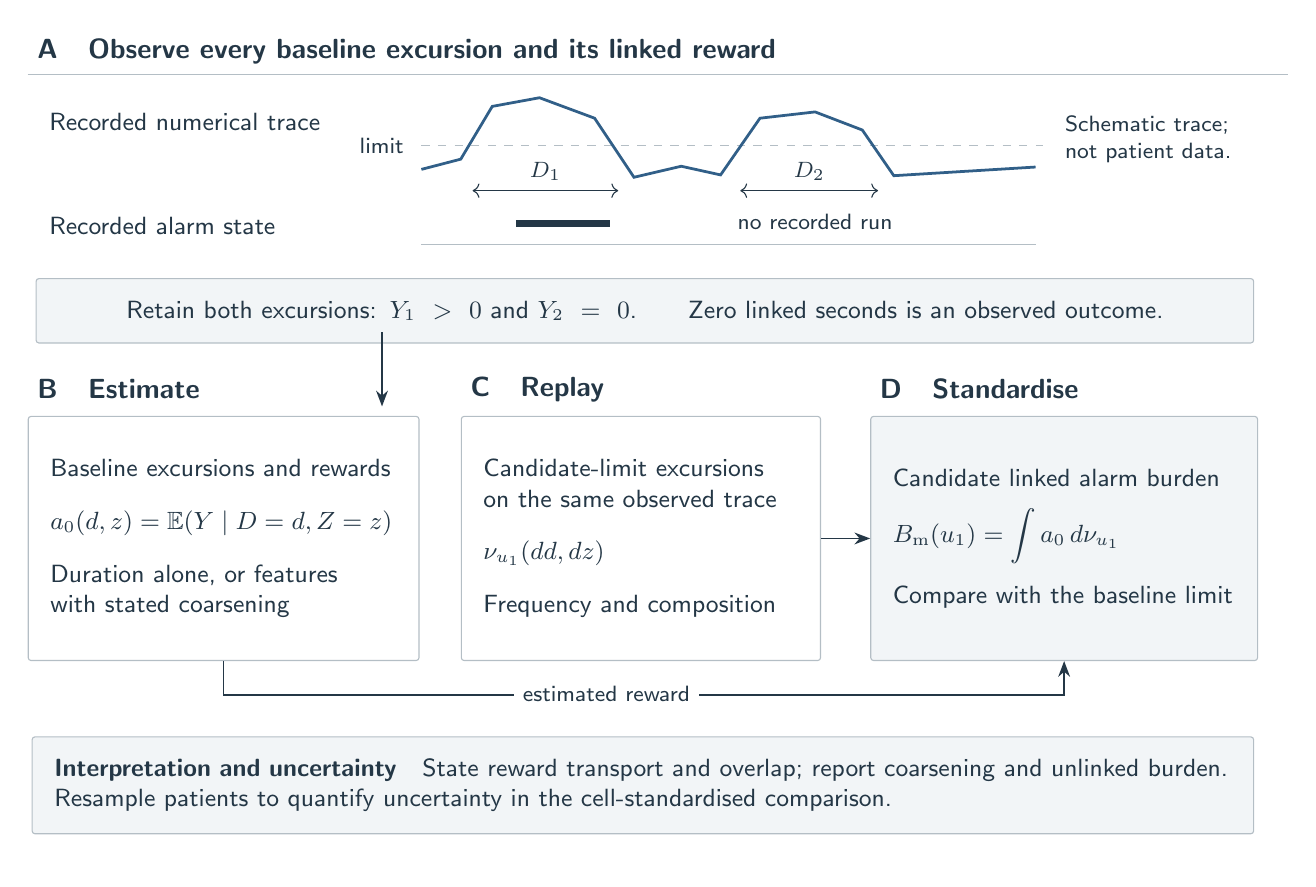
\begin{tikzpicture}[x=1cm,y=1cm,font=\sffamily\small,text=ink,
 box/.style={draw=rule,rounded corners=1pt,fill=white,inner sep=8pt,align=left},
 arrow/.style={-{Stealth[length=2mm]},draw=ink,line width=.65pt}]
\path[use as bounding box] (0,0) rectangle (16.0,10.55);
\node[anchor=west,font=\sffamily\bfseries] at (0,10.25) {A\quad Observe every baseline excursion and its linked reward};
\draw[rule] (0,9.95)--(16,9.95);
\node[anchor=west] at (0.15,9.35) {Recorded numerical trace};
\node[anchor=west] at (0.15,8.03) {Recorded alarm state};
\draw[dashed,rule] (5.0,9.05)--(12.9,9.05);
\node[anchor=east,font=\sffamily\footnotesize] at (4.9,9.05) {limit};
\draw[blue,line width=1pt] (5,8.75)--(5.5,8.88)--(5.9,9.55)--(6.5,9.66)--(7.2,9.40)--(7.7,8.65)--(8.3,8.79)--(8.8,8.68)--(9.3,9.40)--(10,9.48)--(10.6,9.25)--(11,8.67)--(12.8,8.78);
\draw[<->,ink] (5.65,8.48)--node[above,font=\sffamily\footnotesize] {$D_1$} (7.5,8.48);
\draw[<->,ink] (9.05,8.48)--node[above,font=\sffamily\footnotesize] {$D_2$} (10.8,8.48);
\draw[rule,line width=.5pt] (5,7.8)--(12.8,7.8);
\draw[ink,line width=2.6pt] (6.2,8.06)--(7.4,8.06);
\node[font=\sffamily\footnotesize] at (10,8.08) {no recorded run};
\node[anchor=west,font=\sffamily\footnotesize,text width=2.6cm,align=left] at (13.05,9.13) {Schematic trace;\\not patient data.};
\node[box,text width=14.9cm,align=center,anchor=north west,fill=pale] at (0.1,7.37) {Retain both excursions: $Y_1>0$ and $Y_2=0$.\qquad Zero linked seconds is an observed outcome.};
\node[anchor=west,font=\sffamily\bfseries] at (0,5.96) {B\quad Estimate};
\node[box,text width=4.4cm,anchor=north west,minimum height=3.1cm] (est) at (0,5.62) {Baseline excursions and rewards\\[8pt]$a_0(d,z)=\mathbb E(Y\mid D=d,Z=z)$\\[8pt]Duration alone, or features\\with stated coarsening};
\node[anchor=west,font=\sffamily\bfseries] at (5.5,5.96) {C\quad Replay};
\node[box,text width=4.0cm,anchor=north west,minimum height=3.1cm] (rep) at (5.5,5.62) {Candidate-limit excursions\\on the same observed trace\\[8pt]$\nu_{u_1}(dd,dz)$\\[8pt]Frequency and composition};
\node[anchor=west,font=\sffamily\bfseries] at (10.7,5.96) {D\quad Standardise};
\node[box,text width=4.35cm,anchor=north west,minimum height=3.1cm,fill=pale] (out) at (10.7,5.62) {Candidate linked alarm burden\\[7pt]$B_{\mathrm m}(u_1)=\displaystyle\int a_0\,d\nu_{u_1}$\\[7pt]Compare with the baseline limit};
\draw[arrow] (rep.east)--(out.west);
\draw[arrow] (est.south)--++(0,-.43)-| (out.south);
\node[fill=white,font=\sffamily\footnotesize] at (7.35,2.09) {estimated reward};
\draw[arrow] (4.5,6.68)--(4.5,5.74);
\node[box,text width=14.95cm,anchor=north west,fill=pale] at (0.05,1.55) {\textbf{Interpretation and uncertainty}\quad State reward transport and overlap; report coarsening and unlinked burden. Resample patients to quantify uncertainty in the cell-standardised comparison.};
\end{tikzpicture}\end{document}
